\section{Ohm's Law and Equivalent Resistance}

\instructornote{%
By Matt, 2015.  Time: long! ($\sim$100 minutes)

This lab was originally written by Matt Trawick in around 2008, and finally transcribed to Latex for inclusion in this lab manual in 2015.  

This lab builds on ``Introduction to Electric Circuits'' and uses a lot of the same pedagogical approaches.  Don't do this lab as students' first introduction to circuits. 

Equipment notes: 

For the multimeters, have extra fuses on hand, as some fuses will be blown!  But this can be greatly reduced by setting the power supplies ahead of time to a 3 V output, and a current limit of about 400 mA.  (Both fine knobs all the way up, both coarse knobs all the way down, button on "high" range.)

As with the previous circuits lab, I also recommend two pairs of scissors per group, so that each student does their own cutting and folding.  If they both cut, then they will also both fold, and the physical act of folding seems to build a kind of kinesthetic memory for the concept the lab is trying to get across.  Finally, I recommend having students tape down their circuits with masking tape, to avoid spaghetti tangles that are difficult to troubleshoot.
}

\makelabheader %(Space for student name, etc., defined in master.tex)

\bigskip
\textbf{Apparatus}
\begin{itemize}[nosep]
\item digital multimeters (2)
\item DC power supply 
\item one light bulb, in a socket with banana connectors
\item 1 k $\Omega$ resistors (2)
\item 2.2 k$\Omega$ resistors (1)
\item banana jumper wires (at least 5)
\item scissors (2)
\item masking tape
\end{itemize}

\bigskip
\textbf{Introduction:}

In this lab, you will measure both electric currents and potential differences using your digital multimeters (DMMs).  Your instructor will show you how to set up your DMM for each kind of measurement.

\begin{newboxed}
\textit{For all parts of this lab, keep your power supplies set to a voltage of 3.0 volts or less.  Otherwise we'll blow out lots of bulbs and fuses.}
\end{newboxed}

\vspace{0.1 in}

\textbf{Activity 0: Introduction to Multimeters and Resistors}

(1) Use the information in Appendix B and the multimeters at your table to answer the following questions.

\textbf{(a) Measuring Current}
\begin{itemize}
	\item Which input jack is always used when measuring current?
	\answerspace{0.5 in}
	\item How does the second input jack depend on the size of the current? If you're unsure how large the current is, which jack should you start with, and why?
\answerspace{1.0 in}
	\item Where should you set the dial to measure current? How is this setting related to the jack you chose in the previous question?
	\answerspace{1.0 in}
\end{itemize}
\newpage
\textbf{(b) Measuring Voltage}
\begin{itemize}
	\item Which two input jacks should you use to measure voltage?
	\answerspace{0.6 in}
	\item Where should you set the dial when measuring voltage?
	\answerspace{0.6 in}
\end{itemize}

(2) Use the table in Appendix C to find the resistances of the following resistors:
\begin{center}
	\includegraphics[width=0.9\textwidth]{electric_circuits2/resistors.jpg}
	\index{color page}
\end{center}

\textbf{Activity 1: Relationship Between Current and Voltage}

(a) \textit{For the current measurements in this part, start by using your DMM in the 10 Amp or 20 Amp range.  If the current you read is less than 0.4 Amps, you can switch to a mA range.} Connect a single light bulb to your power supply as shown below, measuring both the current $I$ through it and the voltage $\Delta V$ across it as you vary the voltage of the power supply from 0 to 3.0 volts.  Make a graph\footnote{In general, ``plot $A$ \textit{vs.} $B$'' means ``plot $A$ as a function of $B$,'' which implies that thing $B$ should go on the horizontal axis.} of $I$ \textit{vs.} $\Delta V$, for voltages of 0.0, 0.1, 0.3, 0.6, 1.0, 2.0, and 3.0 volts.  Use graphing software (like Excel) for your graph, and then make a pencil sketch of it in the space below.  Is the relationship between $I$ and $\Delta V$ linear? Print your plot and attach it to this unit.

\hspace{0.5in}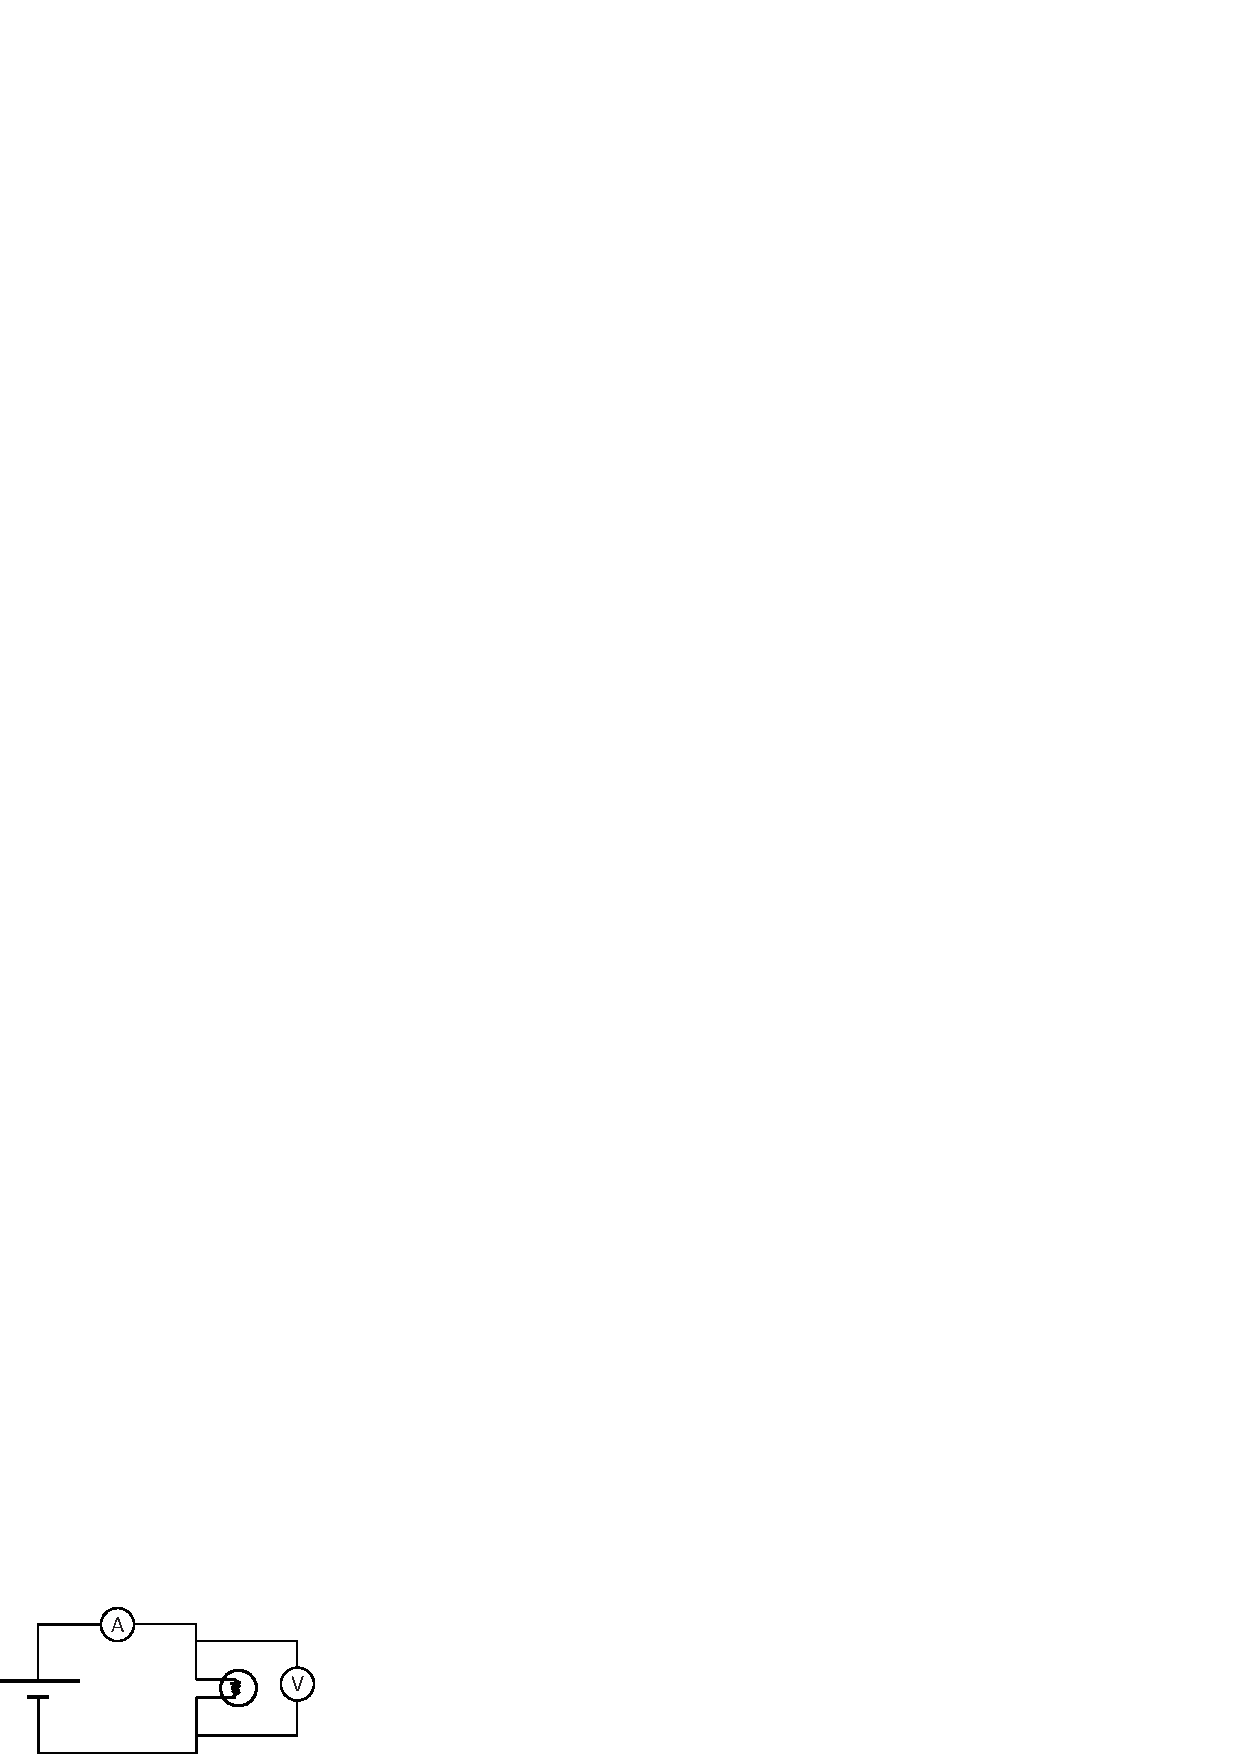
\includegraphics[width=0.3\textwidth]{electric_circuits2/circ_diag1.pdf}
\answerspace{0.5 in}

(b) \textit{For the current measurements in this part, change your DMM to a range between 40 mA and 400 mA if you haven't already.} Repeat the measurements in part (a), replacing the light bulb with a resistor with bands colored brown, black, red, and gold.  Again, make a graph of $I$ \textit{vs.} $\Delta V$.  
Is the relationship between the two linear? Print your plot and attach it to this unit.
\answerspace{1 in}

\newpage
(c) Ohm's law says that for some circuit elements, the current through them is proportional to the voltage across them.  The ratio between the two is the resistance, $R=\Delta V / I$ .  (The unit of resistance is an Ohm ($\Omega$), where 1 Ohm = 1 Volt / 1 Amp.)  Which one of the two things you measured in (a) and (b) follows Ohm's law, and what is its resistance?
\answerspace{0.7 in}

(d) Your DMM allows you to measure resistance directly, without using your power supply.  Disconnect the resistor from your circuit \textit{completely,} and use your DMM to measure its resistance.  (The leads go in the same holes you used to measure voltage, and the function selector should be turned to ``$\Omega$''.)  What is its resistance?
\answerspace{0.5 in}

(e) The light bulb is designed to glow white hot when current flows in it, and the resistance of the tungsten filament depends strongly on temperature.  That's why the bulb doesn't follow Ohm's law.  From your measurements in (a) does the filament's resistance increase or decrease with temperature?
\answerspace{0.6 in}

\textbf{Activity 2: Two Equal Resistors in Series} \par
\nopagebreak
(a) Build the circuit shown below, which has two 1 k$\Omega$ resistors connected in series.  If your power supply is set to 3 volts, what will be the voltage drop $\Delta V$ across each resistor?  Make a prediction, and test your prediction with a measurement.

\begin{minipage}{0.4\textwidth} 
\hspace{0.5in}\includegraphics[width=0.5\textwidth]{electric_circuits2/circ_diag2_bw.pdf}
\end{minipage}
\begin{minipage}{0.59\textwidth} 
\vspace{0.2 in}
Prediction: \hspace{0.4 in} $\Delta V_{R1} =$ \hspace{0.8 in} $\Delta V_{R2}=$
\vspace{0.2 in}

Measurement: \hspace{0.2 in} $\Delta V_{R1} =$ \hspace{0.8 in} $\Delta V_{R2}=$ 
\answerspace{0.2 in}
\end{minipage}

(b) You saw in Activity 1 that the voltage difference across a resistor is proportional to its current, $\Delta V=IR$.  Make a prediction for the current through the resistors in the circuit.  Test your prediction by inserting a current meter into your circuit and measuring it.  

\vspace{0.2 in}
\hspace{0.4 in} Prediction: \hspace{0.4 in} $I =$ 
\vspace{0.2 in}

\hspace{0.4 in} Measurement: \hspace{0.2 in} $I=$ 
\answerspace{0.2 in}

\pagebreak[2]
(c) We can think of the two resistors in series as being equivalent to a single resistor $R_{EQ}$.  What value single resistor $R_{EQ}$ would we have to replace the two 1k$\Omega$ resistors with in order to draw the same current (about 1.5 mA) from the power supply? \par
\nopagebreak
%\begin{center}
\hspace{0.5in}
\includegraphics[width=0.6\textwidth]{electric_circuits2/circ_diag3_bw.pdf}
\vspace{0.1 in}
%\end{center}

\textbf{Activity 3: Two Different Resistors in Series} \par
\nopagebreak
(a) The circuit below shows a 1 k$\Omega$ and 2.2 k$\Omega$ resistor connected in series.  Which resistor carries the larger current? (Or are they the same?)  Check yourself with a measurement.   The 2.2 k$\Omega$ resistor has bands colored red, red, red, gold.

\begin{minipage}{0.4\textwidth} 
\hspace{0.5in}\includegraphics[width=0.6\textwidth]{electric_circuits2/circ_diag4_bw.pdf}
\end{minipage}
\begin{minipage}{0.59\textwidth} 
\vspace{0.2 in}
Prediction: 
\vspace{0.4 in}

Measurement: \ 
\vspace{0.2 in}
\end{minipage}


(b)Which resistor in the circuit above has a larger voltage drop $\Delta V$ across it?   Why?  Check yourself with a measurement.  

\vspace{0.2 in}
\hspace{0.4 in} Prediction:
\vspace{0.2 in}

\hspace{0.4 in} Measurement:  
\vspace{0.2 in}

(c) Imagine replacing the two resistors in series with a single equivalent resistor $R_{EQ}$.  We can write $R_{EQ}$ in terms of the voltage drops across the resistors as
\begin{displaymath}
R_{EQ} = \frac{\Delta V_{EQ}}{I}= \frac{\Delta V_1 +\Delta V_2 }{I}=\frac{\Delta V_1}{I} + \frac{\Delta V_2}{I}
\end{displaymath}
Use the equation above as a start to write a general expression for $R_{EQ}$ in terms of $R_1$ and $R_2$ for two resistors in series.
\begin{displaymath}
\textrm{For resistors in series: } \boxed{R_{EQ} = \phantom{\rule[-0.1in]{1.0in}{.35in}}}
\end{displaymath}

\textbf{Activity 4: Two Resistors in Parallel} \par
\nopagebreak
(a)  The circuit drawn below shows two resistors in parallel.  Which is bigger, $\Delta V_1$ or $\Delta V_2$? (Or are they the same?)

\hspace{0.5 in}\includegraphics[width=0.4\textwidth]{electric_circuits2/circ_diag5_bw.pdf}
\vspace{0.2 in}

\pagebreak
(b) Which resistor in the circuit above has a larger current through it?   Why? 
 
\vspace{0.2 in}
\hspace{0.4 in} Prediction:
\answerspace{0.2 in}

\hspace{0.4 in} Measurement:  
\answerspace{0.2 in}

(c) What are the currents $I_1$ and $I_2$ through the resistors, in terms of $R_1$, $R_2$, and  $\Delta V$? 
\answerspace{0.6in}

(d) Imagine replacing the two resistors in parallel with a single equivalent resistor $R_{EQ}$.   We can write the current through the equivalent resistor as $I_{EQ}=I_1+I_2$.  Starting with the definition $R_{EQ}=  \Delta V \slash I_{EQ}$, derive an expression for $R_{EQ}$ in terms of $R_1$ and $R_2$ for two resistors in parallel.  (It's not the same as for resistors in series!)

\begin{center}
\includegraphics[width=0.7\textwidth]{electric_circuits2/parallel_equiv_bw.pdf}
\answerspace{1 in}
\end{center}

\begin{displaymath}
%\textrm{For resistors in parallel: } \boxed{R_{EQ} = \rule[-0.2in]{0.5in}{0in}\rule[0.3in]{0.5in}{0in}} 
\textrm{For resistors in parallel: } \boxed{R_{EQ} = \phantom{\rule[-0.3in]{1.2in}{.7in}}} 
\end{displaymath}

\textbf{Activity 5: Using Equivalent Resistances to Solve Problems}

\begin{wrapfigure}[8]{r}{0.3\textwidth}
    \vspace{-0.3 in}
    \includegraphics[width=0.29\textwidth]{electric_circuits2/circ_diag6_bw.pdf}
\end{wrapfigure}

%\vspace{0.3 in}
(a) The last page of this lab is a large picture of this circuit.  Cut it out and fold it so that height above the table at each point of the circuit corresponds to electric potential.  

(b) Which two resistors have the same $\Delta V$?  Which two resistors carry the same current $I$?
\answerspace{0.6 in}

(c) Next, we're going to use the idea of equivalent resistances to find the current that flows in each of the resistors in the circuit.  The flow chart on the following page will guide you through it.

\begin{center}
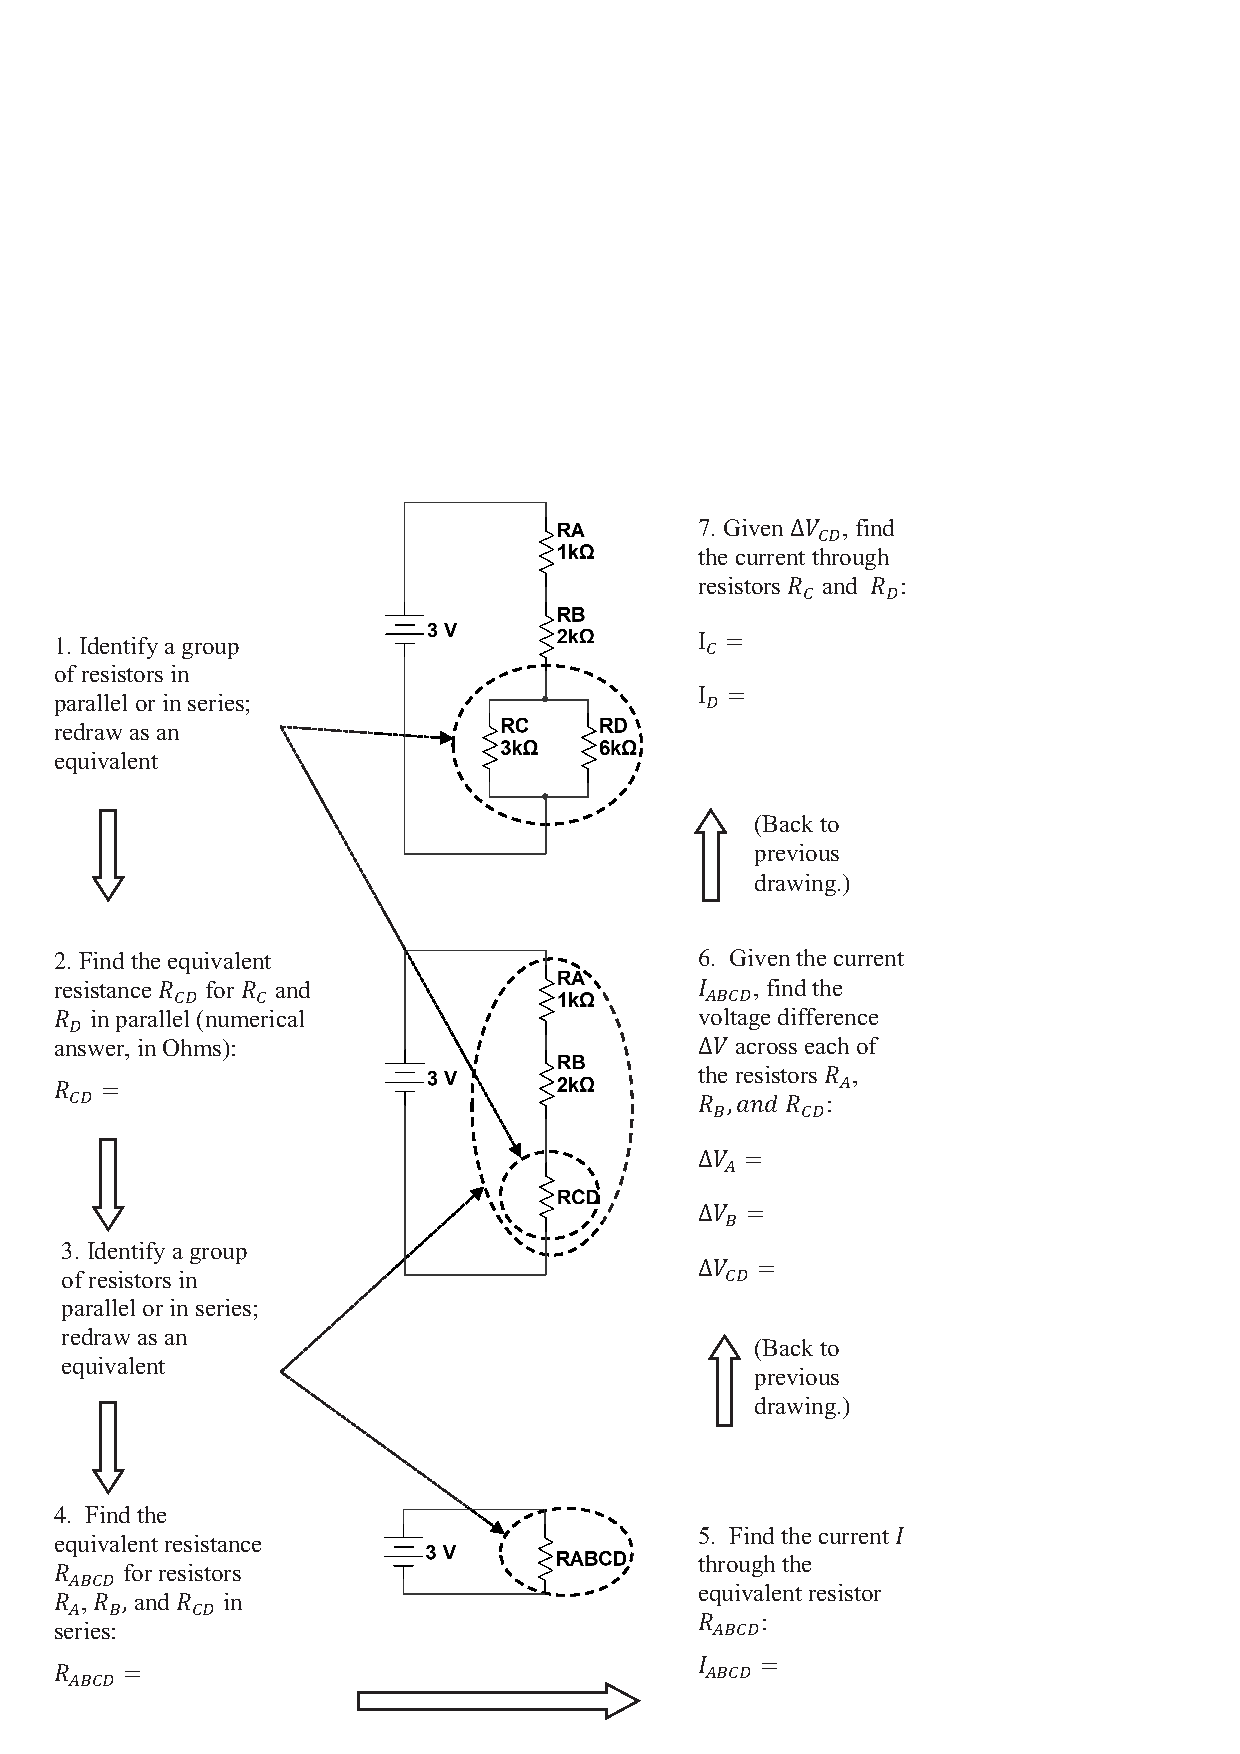
\includegraphics[height=1.0\textheight]{electric_circuits2/step_by_step_circuit.pdf}
\end{center}

\pagebreak
\textbf{Homework Questions} \par
%\nopagebreak
(a) If two resistors are connected in series, do they always carry the same current through them? If not, which one will have the larger current?
\vspace {0.7 in}

(b) If two resistors are connected in series, do they always have the same voltage difference across them?  If not, which one will have the larger voltage difference across it?
\vspace {0.7 in}

(c) If two resistors are connected in parallel, do they always carry the same current through them? If not, which one will have the larger current?
\vspace {0.7 in}

(d) If two resistors are connected in parallel, do they always have the same voltage difference across them?  If not, which one will have the larger voltage difference across it?
\vspace {0.7 in}

\cleardoublepage %force this cutout page to be on the right hand side.
\begin{center}
\includegraphics[width=0.95\textwidth]{electric_circuits2/cutout_page_bw.pdf}
\end{center}

\newpage
[This page left intentionally blank, at least mostly.]
\newpage



